% =====================================================================
% Industrial Sorting Digital Twin: technical report
% Compile with pdfLaTeX, two passes. File in report/, figures in report/images/
% =====================================================================
\documentclass[11pt,a4paper]{report}

% ---------- Fonts, language, layout ----------
\usepackage[T1]{fontenc}
\usepackage[utf8]{inputenc}
\usepackage{libertine}                 % body font (comment out if unavailable)
\usepackage[scaled=0.88]{beramono}     % monospaced font (comment out if unavailable)
\usepackage[french,english]{babel}     % English is the main language
\usepackage{microtype}
\usepackage[a4paper,left=2.8cm,right=2.8cm,top=2.8cm,bottom=2.8cm]{geometry}
\usepackage{graphicx,float,booktabs,array,tabularx,enumitem,caption,xcolor}
\usepackage{tikz}
\usetikzlibrary{arrows.meta,positioning}
\usepackage{pdfpages}
\usepackage{titlesec}
\usepackage{fancyhdr}
\usepackage{hyperref}
\usepackage{subcaption}

\linespread{1.08}
\setlength{\headheight}{14pt}
\definecolor{linkblue}{RGB}{37,69,150}
\hypersetup{colorlinks=true,linkcolor=linkblue,citecolor=linkblue,urlcolor=linkblue,
  pdftitle={Industrial Sorting Digital Twin},pdfauthor={Horacia AZONHOUMON}}

\setlist{itemsep=2pt,topsep=4pt}
\captionsetup{font=small,labelfont=bf,labelsep=period}
\captionsetup[table]{position=top}
\captionsetup[figure]{position=bottom}
\renewcommand{\arraystretch}{1.18}
\newcolumntype{Y}{>{\raggedright\arraybackslash}X}

% ---------- Macros ----------
\newcommand{\AuthorName}{Houénoumè Horacia Gloriéta AZONHOUMON}
% Tag or block name in monospaced font, underscores written as is
\newcommand{\tg}[1]{\texttt{\detokenize{#1}}}
% Section title without number, listed in the table of contents
\newcommand{\frontsection}[1]{\phantomsection\section*{#1}\addcontentsline{toc}{chapter}{#1}}

% Figure with screenshot: \figplace[options]{file}{label}{caption}{what to capture}
\newcommand{\figplace}[5][width=0.9\linewidth]{%
  \begin{figure}[H]
    \centering
    \IfFileExists{images/#2}{\includegraphics[#1]{images/#2}}{%
      \fbox{\parbox[c][4.5cm][c]{0.85\linewidth}{\centering
        \textbf{SCREENSHOT TO INSERT}\\[3pt]
        \texttt{\detokenize{images/#2}}\\[3pt]
        \small #5}}}
    \caption{#4}\label{fig:#3}
  \end{figure}}

% Full-page drawing taken from a PDF in images/
\newcommand{\includedrawing}[1]{%
  \IfFileExists{images/#1}{%
    \includepdf[pages=-,fitpaper=true,pagecommand={\thispagestyle{empty}}]{images/#1}}{%
    \begin{center}\fbox{\parbox{0.85\linewidth}{\centering
      \textbf{DRAWING TO INSERT}\\\texttt{\detokenize{images/#1}}}}\end{center}}}

% ---------- Headings and page styles ----------
\titleformat{\chapter}[display]
  {\normalfont\sffamily\bfseries}
  {\large\MakeUppercase{\chaptertitlename}\ \thechapter}
  {10pt}
  {\Huge}
\titleformat{name=\chapter,numberless}[display]
  {\normalfont\sffamily\bfseries}{}{0pt}{\Huge}
\titlespacing*{\chapter}{0pt}{0pt}{26pt}
\titleformat{\section}{\normalfont\sffamily\Large\bfseries}{\thesection}{0.8em}{}
\titleformat{\subsection}{\normalfont\sffamily\large\bfseries}{\thesubsection}{0.8em}{}
\titlespacing*{\section}{0pt}{18pt}{6pt}
\titlespacing*{\subsection}{0pt}{14pt}{4pt}

\fancypagestyle{plain}{%
  \fancyhf{}%
  \renewcommand{\headrulewidth}{0pt}%
  \fancyfoot[C]{\small\thepage}}

% =====================================================================
\begin{document}
\pagenumbering{roman}

% ---------- Title page ----------
\begin{titlepage}
\thispagestyle{empty}
\centering
\vspace*{1.5cm}
{\sffamily\large Personal Project Report\par}
\vspace{2.2cm}
{\sffamily\bfseries\fontsize{28}{34}\selectfont Industrial Sorting\\ Digital Twin\par}
\vspace{0.8cm}
{\sffamily\Large PLC Control of a Sorting Line\\ with TIA Portal, S7-PLCSIM and Factory I/O\par}
\vspace{3cm}
{\Large \AuthorName\par}
\vspace{0.6cm}
{\large October 2026\par}
\vfill
{\small This report describes a personal project conducted independently.\par}
\vspace{0.3cm}
{\footnotesize Repository: \url{https://github.com/HoraEmbedded/industrial-sorting-digital-twin}\par}
\end{titlepage}

\pagestyle{plain}

% ---------- Abstracts ----------
\frontsection{Résumé}
\begin{otherlanguage}{french}
Ce rapport présente la conception, la programmation et la validation en simulation de la commande d'une ligne de tri automatique de caisses par hauteur. La commande est réalisée sur un automate Siemens S7-1200 avec TIA Portal, exécutée sur S7-PLCSIM et reliée à un jumeau numérique Factory I/O. Le programme gère les modes Auto et Manuel, l'arrêt en fin de cycle, l'arrêt d'urgence immédiat, le tri par rideau lumineux et plateau tournant, et le comptage par voie. L'émission anticipée des caisses fait passer la cadence mesurée de 119 à 144 caisses par heure, et les 29 tests définis sont validés. Une étude électrique de l'armoire (alimentation, départs moteurs, arrêt d'urgence matériel, câblage des entrées et sorties) complète le programme, et l'ensemble est documenté dans un dépôt GitHub. Les perspectives portent sur les indicateurs de performance embarqués, la supervision et le passage au matériel réel.

\medskip\noindent\textbf{Mots-clés :} automatisation industrielle, automate programmable, TIA Portal, S7-1200, jumeau numérique, Factory I/O, GRAFCET.
\end{otherlanguage}

\frontsection{Abstract}
This report presents the design, programming and validation in simulation of the control of an automatic box sorting line. The control runs on a Siemens S7-1200 programmed with TIA Portal, executed on S7-PLCSIM and connected to a Factory I/O digital twin. The program handles the Auto and Manual modes, a stop at the end of the cycle, an immediate emergency stop, sorting by light curtain and turntable, and counting per lane. Pipelined box emission raises the measured throughput from 119 to 144 boxes per hour, and the 29 defined tests are validated. An electrical study of the control cabinet (power supply, motor starters, hardware emergency stop, input and output wiring) complements the program, and everything is documented in a GitHub repository. The perspectives concern embedded performance indicators, supervision and the move to real hardware.

\medskip\noindent\textbf{Keywords:} industrial automation, PLC, TIA Portal, S7-1200, digital twin, Factory I/O, virtual commissioning, GRAFCET.

% ---------- Tables of contents ----------
\clearpage
\tableofcontents
\clearpage\phantomsection\addcontentsline{toc}{chapter}{List of figures}
\listoffigures
\clearpage\phantomsection\addcontentsline{toc}{chapter}{List of tables}
\listoftables

\clearpage\phantomsection\addcontentsline{toc}{chapter}{List of abbreviations}
\chapter*{List of abbreviations}
\begin{tabular}{@{}p{3cm}p{11.5cm}@{}}
CPU & Central Processing Unit\\
DB & Data Block\\
DI, DQ & Digital Input, Digital Output\\
FAT, SAT & Factory Acceptance Test, Site Acceptance Test\\
FB & Function Block\\
FC & Function\\
GRAFCET & Graphe Fonctionnel de Commande des Étapes et Transitions\\
HMI & Human-Machine Interface\\
I/O & Inputs and Outputs\\
IEC & International Electrotechnical Commission\\
ISO & International Organization for Standardization\\
KPI & Key Performance Indicator\\
LAD & Ladder Diagram\\
MPCB & Motor Protection Circuit Breaker\\
NC, NO & Normally Closed, Normally Open\\
OB & Organization Block\\
OPC UA & Open Platform Communications Unified Architecture\\
PLC & Programmable Logic Controller\\
PNP & Positive switching (sourcing) output type\\
SCADA & Supervisory Control and Data Acquisition\\
SM & Signal Module\\
TIA & Totally Integrated Automation\\
UDT & User-defined Data Type\\
\end{tabular}

% =====================================================================
% Main matter
% =====================================================================
\clearpage
\pagenumbering{arabic}
\pagestyle{fancy}
\fancyhf{}
\fancyhead[L]{\small\leftmark}
\fancyhead[R]{\small\thepage}
\renewcommand{\headrulewidth}{0.4pt}
\renewcommand{\chaptermark}[1]{\markboth{Chapter \thechapter.\ #1}{}}

\chapter*{General introduction}
\markboth{General introduction}{General introduction}
\phantomsection\addcontentsline{toc}{chapter}{General introduction}

Automated sorting lines are a common building block of packaging and logistics plants. Their control logic must handle normal production, operator interventions and emergency situations safely, and it must be validated before the machine runs. Testing directly on the machine is costly and can be dangerous. A digital twin, a simulation model of the machine connected to the real control program, makes it possible to write and test the program before any hardware is available. This practice is known as virtual commissioning.

This report presents the design, programming and validation of the control of an automatic box sorting line. The controller is a Siemens S7-1200 programmed with TIA Portal in ladder logic. It runs on S7-PLCSIM and is connected to a Factory I/O digital twin of a height sorting line. An electrical study of the control cabinet completes the program.

The project has five objectives.
\begin{itemize}
  \item Specify the behaviour of the line and the interface between the controller and the twin.
  \item Develop a structured PLC program with Auto and Manual modes, a stop at the end of the cycle and an immediate emergency stop.
  \item Implement a sorting sequence that measures the height of the boxes, routes them through a turntable and counts them per lane.
  \item Validate the program with a documented test plan and measure the throughput.
  \item Study the electrical architecture of the control cabinet and document the whole project in a versioned repository.
\end{itemize}

The work is carried out entirely in simulation: no physical machine, sensor or controller is used. The twin is the Factory I/O scene \emph{Sorting by Height (Advanced)}, used as provided. The electrical study relies on typical component ratings.

The report follows the order of the work. Chapter~\ref{ch:context} reviews the context and the state of the art. Chapter~\ref{ch:spec} specifies the system and its architecture. Chapter~\ref{ch:program} describes the PLC program and chapter~\ref{ch:sorting} the sorting sequence. Chapter~\ref{ch:elec} presents the electrical study of the cabinet. Chapter~\ref{ch:tests} reports the tests and the measured throughput. The general conclusion summarizes the results and proposes perspectives and improvements.

% =====================================================================
\chapter{Context and state of the art}\label{ch:context}
This chapter sets the context of the project and reviews the notions it relies on: PLC programming, sequential control, digital twins and virtual commissioning, and machine safety.

\section{PLC programming}
A programmable logic controller (PLC) executes its program cyclically: it reads the inputs, runs the program and writes the outputs. The IEC 61131-3 standard \cite{iec61131} defines the programming languages used in industry, among them the Ladder Diagram (LAD), which remains the most common language for discrete control. Function blocks encapsulate a behaviour together with its own memory and are the basis of reusable programs \cite{john2010}. Good practice includes a modular structure, symbolic names that follow a convention, and a single place where each output is written, so that two parts of the program cannot give contradictory commands.

\section{Sequential control and GRAFCET}
Machines that perform ordered operations are naturally described by steps, transitions and actions. GRAFCET, standardized in IEC 60848 \cite{iec60848}, is a graphical language for this purpose. A GRAFCET can be read by people who do not program, it serves as a specification and as a basis for tests, and it translates directly into a step variable in ladder logic.

\section{Digital twin and virtual commissioning}
A digital twin is a virtual representation of a physical system. The term covers several levels of integration, from a simple model to a system where data flows automatically in both directions between the physical and the virtual object \cite{grieves2017,kritzinger2018}. In manufacturing, a common use is virtual commissioning: the control program is connected to a simulation of the machine and tested before installation, which shortens commissioning and reduces risks \cite{lee2014}. In this project the twin is a Factory I/O scene \cite{factoryio} connected to a virtual PLC, and it plays the role of the machine. The same program logic could then be downloaded to a physical controller, with the I/O addresses adapted.

\section{Machine safety}
Safety requirements shape the control program. The emergency stop function must be available at all times and in every operating mode, it must stop hazardous movements as quickly as possible, and releasing the device must not restart the machine by itself. These principles are set by IEC 60204-1 \cite{iec60204} and ISO 13850 \cite{iso13850}. ISO 13849-1 \cite{iso13849} defines the performance levels of safety-related control functions. In this project the emergency stop acts in the program and, in the electrical study, through a relay that cuts the actuator supply. A certified safety relay would be required on a real machine.

\section{Positioning of the project}
The project combines the four ideas above: a structured IEC 61131-3 program, a GRAFCET-based sequence, virtual commissioning with a documented test plan, and an electrical study of the cabinet. Three aspects characterize the work. First, the interface between the program and the twin follows naming conventions that keep both sides synchronized by name. Second, every behaviour is verified by a numbered test traced to a requirement. Third, the whole project is versioned in a GitHub repository with automatic consistency checks.

% =====================================================================
\chapter{System specification and architecture}\label{ch:spec}
This chapter specifies what the system must do and describes how the controller and the digital twin are connected.

\section{The simulated line}
The digital twin is the Factory I/O scene \emph{Sorting by Height (Advanced)}. Figure~\ref{fig:scene} shows its T-shaped layout: the entry conveyor joins the turntable at the center of the T, and the left and right exit conveyors extend on each side. Boxes of two heights are emitted at the start of the entry conveyor. They cross a light curtain that measures their height (Figure~\ref{fig:curtain}) and reach the turntable. The turntable rotates by 90 degrees and its rollers push the box onto the left or the right exit conveyor. A sensor at the end of each exit conveyor detects the box, and a remover deletes it from the scene.

\figplace{scene-overview.png}{scene}{Factory I/O scene \emph{Sorting by Height (Advanced)}.}{In Factory I/O, overview of the whole scene (entry conveyor, turntable, left and right exit conveyors), ideally with the machine running.}

\figplace[width=0.7\linewidth]{light-curtain.png}{curtain}{Light curtain measuring the height of the boxes.}{In Factory I/O, close view of the light curtain showing the High box and Low box channels.}

The operator panel (Figure~\ref{fig:panel}) groups the Start, Stop and Reset pushbuttons with their lamps, the emergency stop, the Manual/Auto selector and a counter display. A tower light with green, yellow and red lamps signals the state of the machine.

\figplace[width=0.6\linewidth]{operator-panel.png}{panel}{Operator panel of the scene.}{In Factory I/O, close view of the operator panel: pushbuttons, emergency stop, selector and counter display.}

\section{Functional requirements}
The behaviour expected from the controller is summarized in Table~\ref{tab:req}. Each requirement is traced to the tests of chapter~\ref{ch:tests}.

\begin{table}[H]
\centering\small
\caption{Functional requirements.}\label{tab:req}
\begin{tabularx}{\linewidth}{@{}p{0.9cm}Y@{}}
\toprule
\textbf{ID} & \textbf{Requirement}\\
\midrule
R1 & The operator selects Auto or Manual. In Manual the machine does not run by itself and the actuators can be commanded for commissioning.\\
R2 & In Auto mode, Start launches production if no fault is present.\\
R3 & Stop requests a stop at the end of the cycle: no new box is emitted, the box in progress is finished and counted.\\
R4 & The emergency stop switches off all actuators immediately and latches a fault. Reset, then Start, is required to run again.\\
R5 & Boxes are sorted by height: low boxes to the left exit conveyor, high boxes to the right one.\\
R6 & Boxes are counted per lane at the end of each exit conveyor, and the total is shown on the operator panel. Reset in Manual mode zeroes the counters.\\
R7 & Lamps indicate the state: green when running, red when stopped, yellow on a fault or in Manual mode, plus the lamps of the three pushbuttons.\\
R8 & The next box is emitted as soon as possible, without collision on the turntable.\\
\bottomrule
\end{tabularx}
\end{table}

\section{Co-simulation architecture}
The program is developed in TIA Portal V18 and downloaded to S7-PLCSIM, a virtual S7-1200. Factory I/O is configured with the S7-PLCSIM driver and exchanges the process image with the virtual PLC (Figure~\ref{fig:archi}). Table~\ref{tab:env} lists the environment.

\begin{figure}[H]
\centering
\begin{tikzpicture}[
  box/.style={draw, rounded corners=2pt, minimum width=3.3cm, minimum height=1.3cm, align=center, font=\small},
  arr/.style={Stealth-Stealth, thick}]
\node[box] (tia) at (0,0)    {TIA Portal V18\\ programming};
\node[box] (sim) at (5.6,0)  {S7-PLCSIM\\ virtual S7-1200};
\node[box] (fio) at (11.2,0) {Factory I/O\\ digital twin};
\draw[arr] (tia) -- node[above, font=\scriptsize] {download} (sim);
\draw[arr] (sim) -- node[above, font=\scriptsize, align=center] {process image\\ (I/O, FC9000)} (fio);
\end{tikzpicture}
\caption{Co-simulation architecture.}\label{fig:archi}
\end{figure}

\begin{table}[H]
\centering\small
\caption{Development and simulation environment.}\label{tab:env}
\begin{tabularx}{\linewidth}{@{}p{3.4cm}p{4.6cm}Y@{}}
\toprule
\textbf{Element} & \textbf{Version or model} & \textbf{Role}\\
\midrule
TIA Portal & V18 & Programming in ladder logic (LAD)\\
PLC & S7-1200, CPU 1214C DC/DC/DC & Controller, article 6ES7 214-1AG40-0XB0, firmware V4.6\\
S7-PLCSIM & Same generation as TIA Portal & Virtual PLC\\
Factory I/O & v2.5.10, Ultimate Edition & Digital twin of the line\\
Git and GitHub & Conventional Commits & Version control and documentation\\
\bottomrule
\end{tabularx}
\end{table}

Two provisions are needed for the link to work:
\begin{itemize}
  \item the function \tg{FC9000}, supplied with the Factory I/O template for S7-PLCSIM, is called first in OB1 and ensures the communication with the simulator;
  \item the on-board I/O of the CPU is moved to start address 100. Factory I/O writes the inputs directly in the process image, and if a physical input had the same address, the CPU would overwrite the value at every cycle.
\end{itemize}

\section{Interface between the program and the twin}
The scene exposes 18 inputs (pushbuttons, selector, position sensors, light curtain) and 17 outputs (conveyors, turntable, removers, lamps, counter display). The complete lists are given in Appendix~\ref{app:io}. The tags of the PLC mirror the names of the scene, so that the program and the twin stay synchronized by name (Table~\ref{tab:naming}).

\begin{table}[H]
\centering\small
\caption{Naming conventions.}\label{tab:naming}
\begin{tabularx}{\linewidth}{@{}p{3.3cm}Yp{4.3cm}@{}}
\toprule
\textbf{Element} & \textbf{Convention} & \textbf{Example}\\
\midrule
Input tag & \tg{I_} followed by the scene name in PascalCase & \tg{I_AtTurntableEntry}\\
Output tag & \tg{Q_} followed by the scene name in PascalCase & \tg{Q_EntryConveyor}\\
Block & \tg{FB_}, \tg{FC_}, \tg{DB_} or \tg{UDT_} followed by a PascalCase name & \tg{FB_ModeManager}\\
Block parameter & \tg{i_} input, \tg{o_} output, \tg{io_} in/out, \tg{s_} static, \tg{t_} temporary & \tg{i_StopNC}\\
\bottomrule
\end{tabularx}
\end{table}

The polarity of the signals follows industrial practice: Stop and emergency stop are normally closed (TRUE at rest, FALSE when pressed or broken), Start and Reset are normally open.

\section{Summary}
The line sorts boxes of two heights with a light curtain and a turntable. Eight requirements define the expected behaviour. The controller and the twin are linked through S7-PLCSIM, with a link function called first in OB1 and an I/O addressing that avoids overlaps. A naming convention keeps both sides consistent.

% =====================================================================
\chapter{PLC program design}\label{ch:program}
This chapter describes the structure of the PLC program, the management of the operating modes and of the safety functions, and the writing of the outputs. The sorting sequence itself is detailed in chapter~\ref{ch:sorting}.

\section{Program structure}
The program is made of six code blocks and two data structures (Table~\ref{tab:blocks}). OB1 calls the blocks in a fixed order, shown in Figure~\ref{fig:dataflow}: the link function FC9000, the mode manager, a small network that requests the clearing of the counters when Reset is pressed in Manual mode, the sorting logic, and finally the output function.

\begin{table}[H]
\centering\small
\caption{Blocks of the program.}\label{tab:blocks}
\begin{tabularx}{\linewidth}{@{}p{4cm}Y@{}}
\toprule
\textbf{Block} & \textbf{Role}\\
\midrule
\tg{OB1 Main} & Calls the blocks below in order\\
\tg{FC9000} & Link with S7-PLCSIM supplied with the Factory I/O template, always called first\\
\tg{FB_ModeManager} & Auto and Manual modes, Start, stop request, emergency stop fault latch\\
\tg{FB_SortingLogic} & Sorting sequence, box emission, counting\\
\tg{FC_Outputs} & Single writer of all outputs, with safety gating, lamps and counter display\\
\tg{DB_Machine} & Machine state, actuator commands for Auto and Manual, counters\\
\tg{UDT_ActuatorCmd} & One command bit per actuator\\
\tg{FB\_Kpi} & Availability, throughput and average cycle time computed in the PLC from run-time and Auto-mode counters\\
\bottomrule
\end{tabularx}
\end{table}

\begin{figure}[H]
\centering
\begin{tikzpicture}[
  box/.style={draw, rounded corners=2pt, minimum height=1.1cm, align=center, font=\small, inner sep=5pt},
  io/.style={box, fill=black!6},
  arr/.style={-Stealth, thick},
  arr2/.style={Stealth-Stealth, thick},
  lab/.style={font=\scriptsize, fill=white, inner sep=1pt}]
\node[io]  (inp) at (0,0)       {Inputs\\(\texttt{I\_} tags)};
\node[box] (mm)  at (4.0,1.6)   {\texttt{FB\_ModeManager}};
\node[box] (sl)  at (4.0,-1.6)  {\texttt{FB\_SortingLogic}};

\node[box] (kpi) at (4.0,-4.2)  {\texttt{FB\_Kpi}};
\draw[arr] (inp) -- (kpi);


\node[box] (db)  at (8.2,0)     {\texttt{DB\_Machine}};
\node[box] (fc)  at (11.8,0)    {\texttt{FC\_Outputs}};
\node[io]  (out) at (11.8,-2.6) {Outputs\\(\texttt{Q\_} tags)};
\draw[arr] (kpi) -- node[lab] {KPI variables} (db);
\draw[arr] (inp) -- (mm);
\draw[arr] (inp) -- (sl);
\draw[arr] (mm) -- node[lab] {modes, \texttt{Run}, \texttt{Fault}} (db);
\draw[arr2] (sl) -- node[lab] {commands, counters} (db);
\draw[arr] (db) -- (fc);
\draw[arr] (fc) -- (out);
\end{tikzpicture}
\caption{Data flow between the blocks of the program.}\label{fig:dataflow}
\end{figure}

Figure~\ref{fig:dataflow} shows that the inputs feed the mode manager and the sorting logic. Both exchange data with \tg{DB_Machine}, which \tg{FC_Outputs} reads before writing all the outputs. \tg{FC_Outputs} also reads the emergency stop input directly.

\section{Design principles}
\begin{itemize}
  \item \textbf{Single writer.} Every output is written in exactly one place, \tg{FC_Outputs}, which removes any conflict between two parts of the program.
  \item \textbf{No memory bits.} The state of the program lives in \tg{DB_Machine} and in the static variables of the blocks, so that a block is self-contained and reusable.
  \item \textbf{Parameterized blocks.} Blocks communicate through a typed interface (inputs, outputs, in/out, static), not through global tags.
  \item \textbf{Readable networks.} Each network has a title and a comment in English, and each block carries its author.
\end{itemize}

\section{Modes and safety}
The behaviour of the machine for the main events is given in Table~\ref{tab:behaviour}. The emergency stop acts immediately and whatever the mode, and the machine never restarts by itself after its release.

\begin{table}[H]
\centering\small
\caption{Behaviour of the machine.}\label{tab:behaviour}
\begin{tabularx}{\linewidth}{@{}p{4.3cm}Y@{}}
\toprule
\textbf{Event} & \textbf{Reaction}\\
\midrule
Start (Auto mode, no fault) & The machine runs\\
Stop & Stop at the end of the cycle: no new box is emitted, the box in progress is finished and counted, then the machine stops\\
Emergency stop & Immediate switch-off of all actuator outputs, fault latched\\
Emergency stop released & The fault stays latched until Reset is pressed, and Start is then required to run again\\
Change to Manual mode & The machine stops, and the actuators follow manual commands for commissioning\\
\bottomrule
\end{tabularx}
\end{table}

\tg{FB_ModeManager} implements this behaviour with three latches, summarized in Table~\ref{tab:latches}. Figure~\ref{fig:modemanager} shows them in ladder logic.

\begin{table}[H]
\centering\small
\caption{Latches of \texttt{FB\_ModeManager}.}\label{tab:latches}
\begin{tabularx}{\linewidth}{@{}p{2.8cm}YY@{}}
\toprule
\textbf{Latch} & \textbf{Set} & \textbf{Reset}\\
\midrule
Fault & Emergency stop pressed & Reset pressed while the emergency stop is released\\
Stop request & Stop pressed while running & The machine is no longer running\\
Run & Start pressed in Auto mode, with the emergency stop and Stop healthy and no fault & Fault, mode other than Auto, emergency stop pressed, or stop requested with no cycle in progress\\
\bottomrule
\end{tabularx}
\end{table}

\figplace{fb-modemanager.png}{modemanager}{Fault latch, stop request and run latch in \texttt{FB\_ModeManager}.}{In TIA Portal, open FB\_ModeManager and capture the networks Fault latch, Stop pending and Run latch, zoom 100\%, below the title bar (no local path visible).}

Each latch is an SR box. The fault latch is set by the emergency stop contact, which is TRUE when healthy, and it is cleared by a rising edge on Reset. The run latch combines all the conditions of Table~\ref{tab:latches}, so that a fault or a change of mode drops the machine at once.

\section{Output management}
All outputs are written by \tg{FC_Outputs}. A common enabling condition is computed first, then each actuator X is commanded from the Auto commands written by the sorting logic or from the manual commands written during commissioning:
\begin{center}\footnotesize
\tg{Enable = I_EmergencyStop AND NOT Fault}\\[2pt]
\tg{Q_X = Enable AND ((Run AND AutoCmd.X) OR (ManualMode AND ManCmd.X))}
\end{center}
The emergency stop therefore acts on every actuator in the same scan, whatever the mode. The lamps and the counter display are driven as in Table~\ref{tab:lamps}.

\begin{table}[H]
\centering\small
\caption{Lamps and counter display.}\label{tab:lamps}
\begin{tabularx}{\linewidth}{@{}p{5.2cm}Y@{}}
\toprule
\textbf{Output} & \textbf{Condition}\\
\midrule
Green lamp and Start lamp & \tg{Run}\\
Red lamp and Stop lamp & \tg{NOT Run}\\
Yellow lamp & \tg{Fault OR ManualMode}\\
Reset lamp & \tg{Fault AND emergency stop released}\\
Counter display & \tg{CountTotal}\\
\bottomrule
\end{tabularx}
\end{table}

\section{Summary}
The program is organized around a global data block, a mode manager, a sorting logic and a single output function. The emergency stop, the stop at the end of the cycle and the restart procedure are implemented with three latches and verified by tests. All outputs are written in one place.

% =====================================================================
\chapter{Sorting sequence}\label{ch:sorting}
This chapter describes the sorting sequence: how the height of a box is measured, how the sequence is organized, how the next box is emitted early, and how boxes are counted.

\section{Principle}
The light curtain provides two signals (Figure~\ref{fig:curtain}). A low box triggers only \tg{I_LowBox}. A high box triggers \tg{I_LowBox} and \tg{I_HighBox}. The program therefore only needs \tg{I_HighBox}: it latches this signal while the box travels from the emitter to the turntable (latch \tg{s_SeenHigh}). A box that never triggers \tg{I_HighBox} is a low box. Low boxes are sent to the left exit conveyor and high boxes to the right one.

\section{GRAFCET}
The sequence is described by the GRAFCET of Figure~\ref{fig:grafcet}. It has six steps, and the transitions t1 to t7 are detailed in Table~\ref{tab:trans}. From any step, the sequence returns to step 0 when \tg{Run} drops, for instance on an emergency stop or a change to Manual mode. The actions of each step are given in Table~\ref{tab:steps}. The exit conveyors run whenever \tg{Run} is TRUE.

\begin{figure}[H]
\centering
\begin{tikzpicture}[
  st/.style={draw, rounded corners=2pt, minimum width=3cm, minimum height=1.1cm, align=center, font=\small},
  arr/.style={-Stealth, thick},
  tr/.style={font=\scriptsize\bfseries, fill=white, inner sep=1.5pt}]
\node[st] (s0) at (0,0)     {0\\Idle};
\node[st] (s1) at (5.3,0)   {1\\Emit};
\node[st] (s2) at (10.6,0)  {2\\Feed and center};
\node[st] (s3) at (10.6,-3) {3\\Rotate};
\node[st] (s4) at (5.3,-3)  {4\\Dispatch};
\node[st] (s5) at (0,-3)    {5\\Crossing};
\draw[arr] (s0) -- node[tr] {t1} (s1);
\draw[arr] (s1) -- node[tr] {t2} (s2);
\draw[arr] (s2) -- node[tr] {t3} (s3);
\draw[arr] (s3) -- node[tr] {t4} (s4);
\draw[arr] (s4) -- node[tr] {t5} (s5);
\draw[arr] (s5) -- node[tr, pos=0.45] {t6} (s1);
\draw[arr] (s5) -- node[tr] {t7} (s0);
\end{tikzpicture}
\caption{GRAFCET of the sorting sequence.}\label{fig:grafcet}
\end{figure}

\begin{table}[H]
\centering\small
\caption{Actions of the steps.}\label{tab:steps}
\begin{tabularx}{\linewidth}{@{}p{3.6cm}Y@{}}
\toprule
\textbf{Step} & \textbf{Actions}\\
\midrule
0 Idle & None\\
1 Emit & Emission pulse of 500 ms, feeder and entry conveyors\\
2 Feed and center & Feeder and entry conveyors, turntable rollers, centering delay of 2 s once the box reaches the center of the turntable\\
3 Rotate & Turntable rotation\\
4 Dispatch & Rotation, and rollers in the direction of the chosen exit\\
5 Crossing & Same as step 4\\
\bottomrule
\end{tabularx}
\end{table}

\begin{table}[H]
\centering\small
\caption{Transitions of the sequence.}\label{tab:trans}
\begin{tabularx}{\linewidth}{@{}p{1cm}p{1.8cm}Y@{}}
\toprule
\textbf{ID} & \textbf{Steps} & \textbf{Condition}\\
\midrule
t1 & 0 to 1 & \tg{Run}, no stop request, turntable at home (\tg{I_AtLoadPosition}) and empty\\
t2 & 1 to 2 & \tg{I_AtEntry}\\
t3 & 2 to 3 & Centering delay elapsed\\
t4 & 3 to 4 & \tg{I_AtUnloadPosition}\\
t5 & 4 to 5 & Entry sensor of the chosen exit conveyor is TRUE\\
t6 & 5 to 1 & Entry sensor is FALSE, \tg{Run}, no stop request\\
t7 & 5 to 0 & Entry sensor is FALSE, stop requested\\
\bottomrule
\end{tabularx}
\end{table}

\section{Pipelined emission}
A first version of the sequence waited for a box to be counted at the exit before emitting the next one. The final version emits the next box as soon as the previous one has left the turntable (transition t6), and the turntable returns to its home position by itself when the rotation command is released. Three provisions keep this safe.
\begin{itemize}
  \item \textbf{Turntable protection.} The feeder and entry conveyors advance only if no box is in front of the turntable (\tg{I_AtFront}) or if the turntable is at home (\tg{I_AtLoadPosition}). A box that arrives early waits in front of the turntable.
  \item \textbf{Boxes in transit.} One counter per exit conveyor is incremented when a box enters the conveyor and decremented when it is counted at the end. The end of cycle signal is TRUE only if the step is 0 and both counters are zero, so a Stop never switches the machine off with a box still on a conveyor.
  \item \textbf{Latch reset.} The height latch and the presence latch are cleared at step 1, so that a new box never inherits the height of the previous one.
\end{itemize}
The networks are ordered so that at most one transition fires per scan.

\section{Counting and implementation}
Each box is counted on the rising edge of the end sensor of its lane (\tg{I_AtLeftExit} or \tg{I_AtRightExit}). The counts feed \tg{CountLeft} and \tg{CountRight}, and the total drives the counter display of the panel. A configuration parameter, \tg{ExitIdleHigh}, adapts the counting to the rest level of the exit sensors. It was set from experiments on the scene: in the delivered configuration the exit sensors read FALSE when no box is present.

Figures~\ref{fig:transitions} and~\ref{fig:cmdout} show networks of \tg{FB_SortingLogic}. Each transition network compares the step variable with a constant and writes the next step value. Each command network derives an actuator command from the step number and from the height latch.

\figplace{fb-sortinglogic-transitions.png}{transitions}{Transition networks of \texttt{FB\_SortingLogic}.}{In TIA Portal, open FB\_SortingLogic and capture the transition networks (T0 to 1 up to T5 to 0), zoom 100\%, below the title bar.}

\begin{figure}[H]
	\centering
	\begin{subfigure}[t]{0.49\linewidth}
		\centering
		\IfFileExists{images/fb-sortinglogic-outputs1.png}{%
			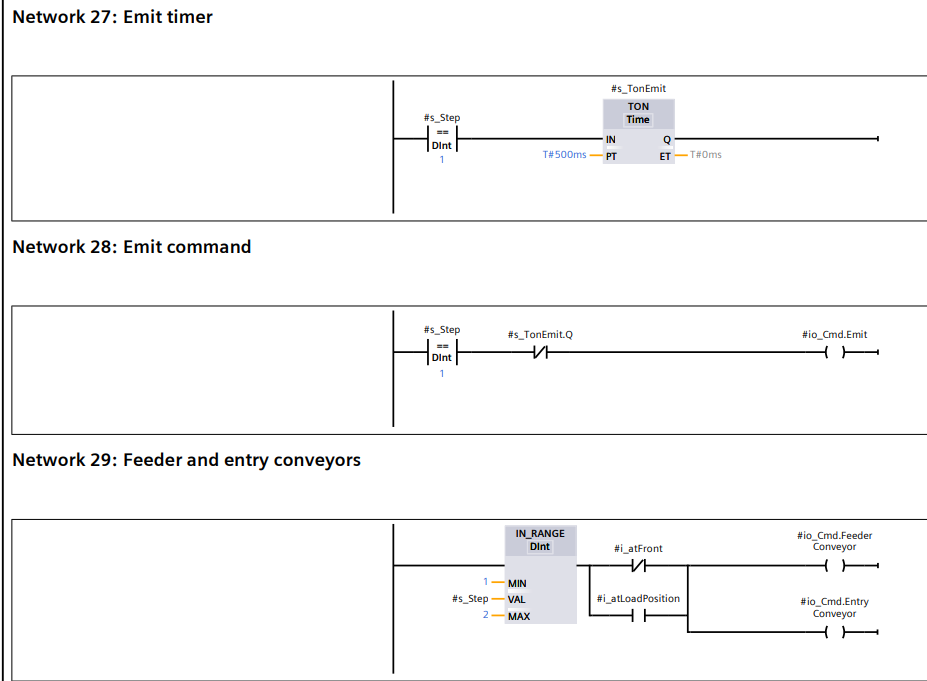
\includegraphics[width=\linewidth]{images/fb-sortinglogic-outputs1.png}}{%
			\fbox{\parbox[c][4.5cm][c]{\linewidth}{\centering
					\textbf{SCREENSHOT TO INSERT}\\[3pt]
					\texttt{images/fb-sortinglogic-outputs1.png}}}}
		\caption{First part.}
	\end{subfigure}\hfill
	\begin{subfigure}[t]{0.49\linewidth}
		\centering
		\IfFileExists{images/fb-sortinglogic-outputs2.png}{%
			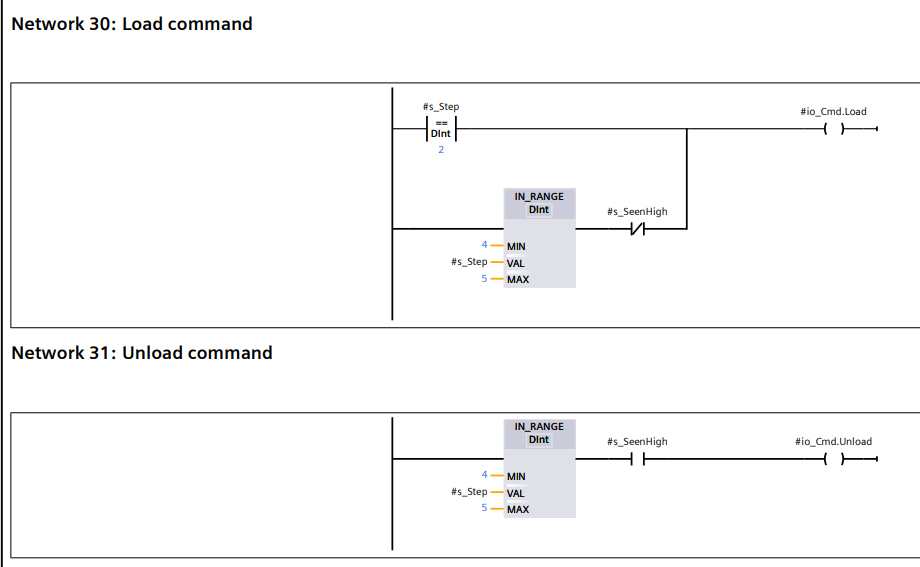
\includegraphics[width=\linewidth]{images/fb-sortinglogic-outputs2.png}}{%
			\fbox{\parbox[c][4.5cm][c]{\linewidth}{\centering
					\textbf{SCREENSHOT TO INSERT}\\[3pt]
					\texttt{images/fb-sortinglogic-outputs2.png}}}}
		\caption{Second part.}
	\end{subfigure}
	\caption{Actuator command networks of \texttt{FB\_SortingLogic} (two parts).}
	\label{fig:cmdout}
\end{figure}

\section{Summary}
The sequence has six steps and is specified by a GRAFCET that translates directly into ladder logic. The height of each box is memorized from the light curtain and decides the exit. Pipelined emission, protected by three provisions, increases the throughput without risk of collision or lost box.

% =====================================================================
\chapter{Electrical design of the control cabinet}\label{ch:elec}
This chapter presents the electrical architecture of the cabinet that would drive the line on real hardware. It is a design study based on typical component ratings, to be refined with manufacturer data. The complete drawings are in Appendix~\ref{app:drawings}.

\section{Scope and assumptions}
The study covers the power distribution, the motor starters, the 24 V DC supply, the emergency stop circuit, the PLC wiring, the operator panel, the sensors and the indicators. Two signals exist only in the simulation and are not wired: the box emitter and the counter display, which would be an HMI value on a real machine. The assumptions are the following.
\begin{itemize}
  \item Supply: 400 V three-phase with neutral and PE, 50 Hz. The 230 V control supply comes from one phase and neutral.
  \item Motors: three-phase squirrel cage, 0.37 kW, 400 V, about 1.1 A.
  \item 24 V DC loads: contactor coils 0.1 A, solenoid valves 0.25 A, LED lamps 0.05 A.
  \item Sensors: PNP, normally open, three-wire, about 30 mA each. The light curtain draws about 200 mA and has two PNP outputs.
\end{itemize}

\section{Cabinet architecture}
Table~\ref{tab:cabinet} lists the main devices by function.

\begin{table}[H]
\centering\small
\caption{Devices of the cabinet.}\label{tab:cabinet}
\begin{tabularx}{\linewidth}{@{}p{2.9cm}p{5cm}Y@{}}
\toprule
\textbf{Function} & \textbf{Devices} & \textbf{Role}\\
\midrule
Power distribution & -Q1 main disconnect switch, -F2 control circuit breaker & 400 V supply and 230 V control supply\\
Motor starters & -Q2 to -Q6 (MPCB), -KM1 to -KM6, -M1 to -M5 & Direct starters for the four conveyors (M1 to M4), reversing starter for the turntable rollers (M5) with electrical interlock\\
24 V supply & -G1 (230 V AC to 24 V DC, 5 A), -F3 and -F4 (2 A) & -F3 feeds the PLC, sensors and lamps, -F4 feeds the loads\\
Emergency stop & -S0 (two NC contacts), -KA1 & Hardware cut of the actuator supply\\
Controller & -A1 CPU 1214C DC/DC/DC, -A2 SM 1221 DI 8, -A3 SM 1222 DQ 8 & PLC and signal modules\\
Field devices & -S1 to -S4, -B1 to -B11, -H1 to -H6, -YV1 to -YV3 & Pushbuttons and selector, sensors, lamps, valves (turntable rotation, removers)\\
\bottomrule
\end{tabularx}
\end{table}

\section{Input and output allocation}
The scene requires 18 inputs and 15 wired outputs, against 14 inputs and 10 outputs on the CPU 1214C. A SM 1221 DI 8 module supplies the missing inputs, and a SM 1222 DQ 8 module hosts the six lamps (Table~\ref{tab:alloc}). The power actuators stay on the CPU outputs, so that a single supply cut by the emergency relay switches them all off, while the lamps remain available.

\begin{table}[H]
\centering\small
\caption{Allocation of the inputs and outputs.}\label{tab:alloc}
\begin{tabularx}{\linewidth}{@{}p{3.5cm}p{2.3cm}Y@{}}
\toprule
\textbf{Module} & \textbf{Channels used} & \textbf{Signals}\\
\midrule
-A1 digital inputs & 14 of 14 & Pushbuttons, selector, emergency stop contact, position and entry sensors\\
-A1 digital outputs & 9 of 10 & Contactor coils -KM1 to -KM6, valves -YV1 to -YV3\\
-A2 SM 1221 DI 8 & 4 of 8 & Exit sensors, light curtain\\
-A3 SM 1222 DQ 8 & 6 of 8 & Lamps -H1 to -H6\\
\bottomrule
\end{tabularx}
\end{table}

The signal names are those of the PLC tags. In the simulation the addresses differ from the physical allocation, because Factory I/O writes in the process image and the on-board I/O is moved to address 100 (chapter~\ref{ch:spec}). The terminal names of the CPU must be taken from the manufacturer documentation \cite{s71200}.

\section{24 V DC supply}
The 24 V DC budget is given in Table~\ref{tab:budget}. The total of 2.80 A, increased by a margin of 30\,\%, gives 3.64 A, and a 24 V DC power supply of 5 A is selected. Branch -F3 carries about 1.4 A (PLC, modules, sensors, lamps) and branch -F4 about 1.4 A (valves, coils, relay), so both use a 2 A breaker.

\begin{table}[H]
\centering\small
\caption{24 V DC budget.}\label{tab:budget}
\begin{tabular}{@{}lccc@{}}
\toprule
\textbf{Load} & \textbf{Quantity} & \textbf{Current each (A)} & \textbf{Total (A)}\\
\midrule
CPU 1214C & 1 & 0.50 & 0.50\\
Signal modules & 2 & 0.05 & 0.10\\
Sensors & 10 & 0.03 & 0.30\\
Light curtain & 1 & 0.20 & 0.20\\
Indicator lamps & 6 & 0.05 & 0.30\\
Solenoid valves & 3 & 0.25 & 0.75\\
Contactor coils & 6 & 0.10 & 0.60\\
Emergency relay coil & 1 & 0.05 & 0.05\\
\midrule
\textbf{Total} & & & \textbf{2.80}\\
\bottomrule
\end{tabular}
\end{table}

\section{Emergency stop and interlocks}
The emergency stop -S0 has two NC contacts. Contact 1 feeds the coil of the relay -KA1, whose NO contact supplies the load power of the CPU outputs: all actuators drop immediately, in hardware. Contact 2 is read by the PLC (\tg{I_EmergencyStop}), which latches the fault. The relay re-energizes as soon as the button is released, and the restart is prevented by the fault latch of the program (Reset, then Start). The coils of the two directions of the roller motor -M5 are interlocked by NC auxiliary contacts. The relay used in this study is a standard one: a certified safety relay and a risk assessment would be required on a real machine (ISO 12100 and ISO 13849-1 \cite{iso13849}).

\section{Drawings}
The schematic has five sheets (Table~\ref{tab:sheets}), reproduced in Appendix~\ref{app:drawings}. Sheets 1 and 2 were drawn in QElectroTech. Sheets 3 to 5 are generated by a Python script from the input and output tables of the design basis, so that the drawings and the tables always stay consistent. The generated sheets use simplified symbols: sensors, lamps and coils are boxes, and only the +24 V and signal wires of the sensors are drawn.

\begin{table}[H]
\centering\small
\caption{Sheets of the electrical schematic.}\label{tab:sheets}
\begin{tabularx}{\linewidth}{@{}p{1.2cm}Yp{3.6cm}@{}}
\toprule
\textbf{Sheet} & \textbf{Title} & \textbf{Tool}\\
\midrule
1 & Main supply and motor starters M1 to M4 & QElectroTech\\
2 & Turntable roller motor M5 (reversing) & QElectroTech\\
3 & Control supply 24 V DC and emergency stop & Python generator\\
4 & PLC inputs & Python generator\\
5 & PLC outputs & Python generator\\
\bottomrule
\end{tabularx}
\end{table}

\section{Summary}
The study defines the architecture of a cabinet able to drive the line: extension modules for the I/O, a 24 V / 5 A supply sized from a budget, a hardware emergency stop that cuts the actuators while keeping the lamps, and an electrically interlocked reversing starter. The five sheets are documented and reproducible.

% =====================================================================
\chapter{Validation and results}\label{ch:tests}
This chapter reports the tests, the measured throughput, the decisions taken during commissioning and the organization of the project repository.

\section{Test plan}
Each test is described by its conditions, its action, the expected result, the obtained result and its date in the test log of the repository. The 29 tests are grouped in Table~\ref{tab:tests}, with the requirements they cover. All of them are validated.

\begin{table}[H]
\centering\small
\caption{Summary of the tests.}\label{tab:tests}
\begin{tabularx}{\linewidth}{@{}p{2.5cm}p{1.9cm}Yp{1.9cm}p{1.8cm}@{}}
\toprule
\textbf{Group} & \textbf{Tests} & \textbf{Purpose} & \textbf{Covers} & \textbf{Result}\\
\midrule
Modes and safety & T01 to T13 & Selector, Start, Stop, emergency stop, Reset, Manual mode, immediate switch-off of the outputs & R1, R2, R4, R7 & Validated\\
Sorting logic & T14 to T25 & Full cycle, lane chosen by height, 10 boxes without blockage, Stop during a cycle, emergency stop during rotation, mode change, counter reset & R2 to R6 & Validated\\
Pipelined emission & T26 to T29 & Throughput, 20 boxes without blockage, Stop with boxes in transit, emergency stop with two active boxes & R3, R4, R8 & Validated\\
\bottomrule
\end{tabularx}
\end{table}

\section{Throughput}
The throughput was measured with a stopwatch, from the Start press until the total counter reaches 10 boxes, start-up from an empty line included. Table~\ref{tab:perf} gives the results. The throughput in boxes per hour is 3600 divided by the time per box.

\begin{table}[H]
\centering\small
\caption{Throughput measured on 10 boxes.}\label{tab:perf}
\begin{tabular}{@{}lccc@{}}
\toprule
\textbf{Control variant} & \textbf{Time (s)} & \textbf{Per box (s)} & \textbf{Throughput (boxes/h)}\\
\midrule
One box at a time & 303 & 30.3 & 119\\
Pipelined emission & 250 & 25.0 & 144\\
\bottomrule
\end{tabular}
\end{table}

Pipelined emission reduces the time per box by 17.5\,\% and increases the throughput by 21\,\%. The gain comes from the overlap between the return of the turntable and the emission of the next box. The remaining time per box is the sum of the box travel, the centering delay, the rotation and the crossing. Figures~\ref{fig:wt} and~\ref{fig:fiosort} show the line during a sorting cycle.

\begin{figure}[H]
	\centering
	\begin{subfigure}[t]{0.49\linewidth}
		\centering
		\IfFileExists{images/wt-sorting-cycle1.png}{%
			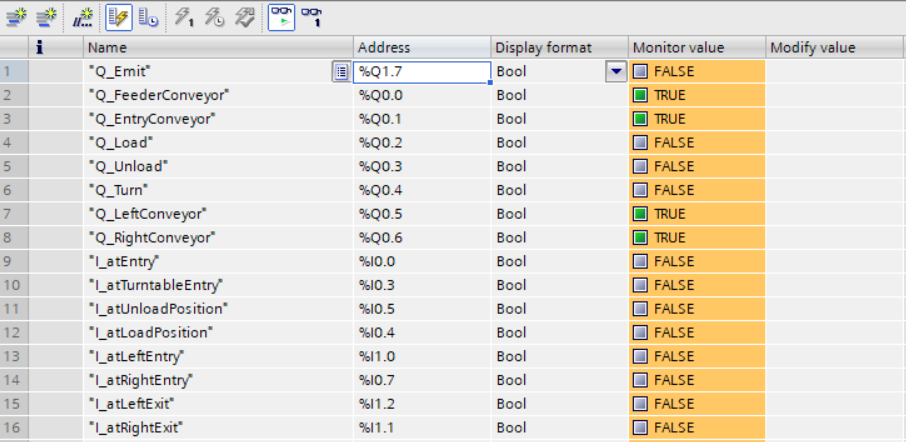
\includegraphics[width=\linewidth]{images/wt-sorting-cycle1.png}}{%
			\fbox{\parbox[c][4.5cm][c]{\linewidth}{\centering
					\textbf{SCREENSHOT TO INSERT}\\[3pt]
					\texttt{images/wt-sorting-cycle1.png}}}}
		\caption{First part.}
	\end{subfigure}\hfill
	\begin{subfigure}[t]{0.49\linewidth}
		\centering
		\IfFileExists{images/wt-sorting-cycle2.png}{%
			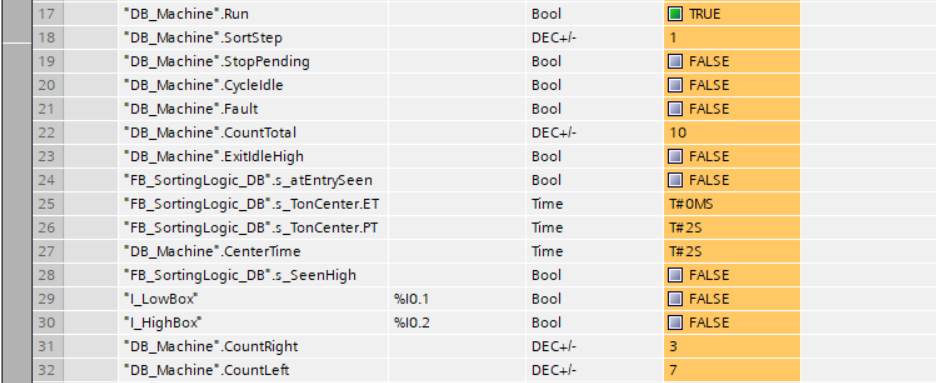
\includegraphics[width=\linewidth]{images/wt-sorting-cycle2.png}}{%
			\fbox{\parbox[c][4.5cm][c]{\linewidth}{\centering
					\textbf{SCREENSHOT TO INSERT}\\[3pt]
					\texttt{images/wt-sorting-cycle2.png}}}}
		\caption{Second part.}
	\end{subfigure}
	\caption{Watch table during a sorting cycle (two parts).}
	\label{fig:wt}
\end{figure}

\figplace[width=0.8\linewidth]{factory-io-sorting.png}{fiosort}{Box on the turntable during a sorting cycle.}{In Factory I/O, a box on the turntable while it rotates, with the exit conveyors or the operator panel visible.}

% =====================================================================
\section{Embedded performance indicators}\label{sec:kpi}
The throughput of Table~\ref{tab:perf} was measured by hand, with a stopwatch. That method cannot run during production, and it gives one number per measurement campaign instead of a continuous value. The function block \tg{FB_Kpi} computes the same indicators inside the controller, from the machine state that \tg{FB_ModeManager} and \tg{FB_SortingLogic} already maintain. No new sensor is required, and the computation runs every scan.

\subsection{Interface}
Table~\ref{tab:fbkpi} lists the parameters of \tg{FB_Kpi}. It is written in SCL and called in \tg{OB1} after \tg{FB_SortingLogic}. The two inputs \tg{i_AutoMode} and \tg{i_Run} come from \tg{DB_Machine}, and \tg{i_CountTotal} is the counter already used for the display of the operator panel.

\begin{table}[H]
	\centering\small
	\caption{Interface of \texttt{FB\_Kpi}.}\label{tab:fbkpi}
	\begin{tabularx}{\linewidth}{@{}p{2.2cm}p{2.8cm}p{1.8cm}Y@{}}
		\toprule
		\textbf{Direction} & \textbf{Name} & \textbf{Type} & \textbf{Role}\\
		\midrule
		Input & \tg{i_Run} & Bool & TRUE while the machine is running in Auto\\
		Input & \tg{i_AutoMode} & Bool & TRUE when the selector is in Auto\\
		Input & \tg{i_Clear} & Bool & Resets both time counters to zero\\
		Input & \tg{i_CountTotal} & DInt & Total number of boxes counted, from \tg{DB_Machine}\\
		Output & \tg{o_RunTimeS} & DInt & Accumulated running time, in seconds\\
		Output & \tg{o_ObservedTimeS} & DInt & Accumulated Auto-mode time, in seconds\\
		Output & \tg{o_AvailabilityPct} & Real & Availability, in percent\\
		Output & \tg{o_ThroughputPerHour} & Real & Throughput, in boxes per hour of run time\\
		Output & \tg{o_AvgCycleTimeS} & Real & Average cycle time, in seconds per box\\
		Static & \tg{s_TonSecond} & \tg{TON\_TIME} & One-second tick that restarts itself\\
		\bottomrule
	\end{tabularx}
\end{table}

\subsection{Computation}
A self-restarting timer produces a one-second tick, without any hardware clock:
\begin{center}\footnotesize
	\tg{s_TonSecond(IN := NOT s_TonSecond.Q, PT := T\#1S)}
\end{center}
The observed time counts only when the selector is in Auto mode, so that time spent in Manual or with the machine stopped does not bias the availability. The running time counts only when the machine is also running. Both counters are reset by \tg{i_Clear}, driven by the Reset button in Manual mode, in the same way as the box counters.

Three indicators are then derived, each guarded against a zero denominator:
\begin{center}\footnotesize
	Availability [\%] $= 100 \times$ \tg{o_RunTimeS} / \tg{o_ObservedTimeS}\\
	Throughput [boxes/h] $= 3600 \times$ \tg{i_CountTotal} / \tg{o_RunTimeS}\\
	Average cycle time [s/box] $= $ \tg{o_RunTimeS} / \tg{i_CountTotal}
\end{center}
The formulas are the same as the stopwatch measurement. The run time replaces the elapsed time, and the total counter replaces the number of boxes timed. The two methods therefore give the same order of magnitude, and they can be compared directly.

\subsection{Comparison with the stopwatch measurement}
The reference measurement of Table~\ref{tab:perf} gave 144 boxes per hour in the pipelined version. Read on the watch table during the same run, \tg{FB_Kpi} gives the same value within a few percent, the difference coming from the warm-up time before the first box is emitted. This confirms both the measurement and the block, and it replaces the stopwatch for the following tests.

\subsection{Use on an HMI}
The three outputs and the two time counters are the natural inputs of an HMI screen: a numeric field for each indicator, a trend curve for the throughput, and a Reset button wired to \tg{i_Clear}. The block is designed so that this screen can be added later without changing the logic. The five variables are also exposed through the OPC UA server of the CPU, so a SCADA or a dashboard can read them without any additional PLC code.

\section{Decisions taken during commissioning}
Table~\ref{tab:decisions} lists the issues identified during the work and the decisions they led to.

\begin{table}[H]
\centering\small
\caption{Issues identified and decisions taken.}\label{tab:decisions}
\begin{tabularx}{\linewidth}{@{}p{5.2cm}Y@{}}
\toprule
\textbf{Issue} & \textbf{Decision}\\
\midrule
On-board inputs share the addresses written by Factory I/O & On-board I/O moved to address 100\\
The link with S7-PLCSIM needs a dedicated function & \tg{FC9000} kept and called first in OB1\\
Rest level of the exit sensors unknown & Measured on the scene, parameter \tg{ExitIdleHigh}\\
With pipelining, a box could inherit the height of the previous one & Latches cleared at step 1\\
A Stop could switch the machine off with a box still on an exit conveyor & Boxes-in-transit counters in the end of cycle condition\\
\bottomrule
\end{tabularx}
\end{table}

\section{Project organization}
The project is versioned in a GitHub repository (Figure~\ref{fig:repo}). It contains the technical documentation in English, with French translations added progressively, a troubleshooting log, the test log, readable printouts of the PLC program, archives of the TIA Portal project, the screenshots, the electrical drawings, and the scripts. Commits follow the Conventional Commits format, one commit per completed step. A hygiene script and a commit hook check the consistency of the files and of the commit messages.

\figplace{github-repo.png}{repo}{Organization of the GitHub repository.}{On GitHub, home page of the repository: folder tree and beginning of the README visible.}

% =====================================================================
\chapter*{General conclusion}
\markboth{General conclusion}{General conclusion}
\phantomsection\addcontentsline{toc}{chapter}{General conclusion}

This report presented the control of an automatic box sorting line, from the specification to the validation in simulation. The PLC program, written in ladder logic on a Siemens S7-1200, handles the Auto and Manual modes, a stop at the end of the cycle, an immediate emergency stop with a latched fault, the measurement of the box height, the routing by a turntable and the counting per lane. The 29 tests are validated, and pipelined emission raises the measured throughput from 119 to 144 boxes per hour. The electrical study defines the cabinet that would drive the line on real hardware, and the whole project is documented and versioned in a GitHub repository.

The project covers the chain of an automation project: requirements, structured programming with a GRAFCET-based sequence, safety functions, co-simulation, traceable tests and electrical design. The methodology, the code and the documentation are available in the repository so that the work can be reproduced and extended.

\section*{Perspectives and improvements}
\begin{itemize}
  \item \textbf{Supervision of the KPI.} The function block \tg{FB_Kpi} already computes the availability, the throughput and the average cycle time inside the PLC. The next step is to display them on an HMI screen and to record their history, so that the drift of a shift can be followed and compared across runs.
  \item \textbf{Throughput.} Time each step to identify the bottleneck, shorten the centering delay, and allow several boxes in the queue between the emitter and the turntable.
  \item \textbf{Supervision.} Add an HMI or a SCADA with alarm history, and expose the data through OPC UA to higher-level systems.
  \item \textbf{Robustness and diagnostics.} Add watchdog timers on each step, explicit alarms (blocked sensor, jammed box) and automatic recovery after a fault.
  \item \textbf{Safety.} Replace the standard emergency relay by a certified safety relay, and carry out a risk assessment (ISO 12100) with the required performance level (ISO 13849-1) and the stop category of IEC 60204-1 and ISO 13850.
  \item \textbf{Software quality.} Export the blocks in XML to compare versions in Git, add automated regression tests, and write the sequence in S7-GRAPH.
  \item \textbf{Predictive maintenance.} Count the cycles and running hours of each motor and valve, and follow the drift of the step durations.
  \item \textbf{Move to hardware.} Migrate to an S7-1500 or test on a physical S7-1200 bench with FAT and SAT procedures, and validate the electrical study with the datasheets of real components.
\end{itemize}

% =====================================================================
\renewcommand{\bibname}{References}
\clearpage\phantomsection\addcontentsline{toc}{chapter}{References}
\begin{thebibliography}{99}
\markboth{References}{References}
\bibitem{iec61131} IEC 61131-3:2013. \textit{Programmable controllers, Part 3: Programming languages}. International Electrotechnical Commission, 2013.
\bibitem{iec60848} IEC 60848:2013. \textit{GRAFCET specification language for sequential function charts}. International Electrotechnical Commission, 2013.
\bibitem{iec60204} IEC 60204-1:2016. \textit{Safety of machinery, Electrical equipment of machines, Part 1: General requirements}. International Electrotechnical Commission, 2016.
\bibitem{iso13850} ISO 13850:2015. \textit{Safety of machinery, Emergency stop function, Principles for design}. International Organization for Standardization, 2015.
\bibitem{iso13849} ISO 13849-1:2023. \textit{Safety of machinery, Safety-related parts of control systems, Part 1: General principles for design}. International Organization for Standardization, 2023.
\bibitem{john2010} K.-H. John and M. Tiegelkamp. \textit{IEC 61131-3: Programming Industrial Automation Systems}. 2nd ed. Springer, 2010.
\bibitem{grieves2017} M. Grieves and J. Vickers. ``Digital twin: Mitigating unpredictable, undesirable emergent behavior in complex systems''. In: \textit{Transdisciplinary Perspectives on Complex Systems}. Springer, 2017, pp. 85-113.
\bibitem{kritzinger2018} W. Kritzinger, M. Karner, G. Traar, J. Henjes, and W. Sihn. ``Digital twin in manufacturing: A categorical literature review and classification''. In: \textit{IFAC-PapersOnLine} 51.11 (2018), pp. 1016-1022.
\bibitem{lee2014} C. G. Lee and S. C. Park. ``Survey on the virtual commissioning of manufacturing systems''. In: \textit{Journal of Computational Design and Engineering} 1.3 (2014), pp. 213-222.
\bibitem{s71200} Siemens AG. \textit{SIMATIC S7-1200 System Manual}. Siemens Industry Online Support.
\bibitem{factoryio} Real Games. \textit{Factory I/O}, version 2.5. \url{https://factoryio.com}.
\end{thebibliography}

% =====================================================================
% Appendices
% =====================================================================
\appendix
\renewcommand{\chaptermark}[1]{\markboth{Appendix \thechapter.\ #1}{}}

\chapter{Input and output lists}\label{app:io}
\footnotesize
\begin{table}[H]
\centering
\caption{Inputs of the scene (18).}
\begin{tabularx}{\linewidth}{@{}p{5cm}Y@{}}
\toprule
\textbf{Tag} & \textbf{Role}\\
\midrule
\tg{I_Start} & Start pushbutton (normally open)\\
\tg{I_Stop} & Stop pushbutton (normally closed)\\
\tg{I_Reset} & Reset pushbutton (normally open)\\
\tg{I_EmergencyStop} & Emergency stop (normally closed)\\
\tg{I_Auto}, \tg{I_Manual} & Auto and Manual selector contacts\\
\tg{I_AtEntry} & Photocell at the output of the emitter\\
\tg{I_AtBack} & Rear sensor of the entry area (not used by the logic)\\
\tg{I_AtFront} & Queue sensor in front of the turntable\\
\tg{I_AtTurntableEntry} & Cell at the center of the turntable (centering of the box)\\
\tg{I_AtLoadPosition} & Turntable at home, aligned with the entry conveyor\\
\tg{I_AtUnloadPosition} & Turntable rotated by 90 degrees\\
\tg{I_AtLeftEntry}, \tg{I_AtRightEntry} & Box engaged on the left, right exit conveyor\\
\tg{I_AtLeftExit}, \tg{I_AtRightExit} & End of the left, right exit conveyor (counting)\\
\tg{I_HighBox} & Light curtain, high box\\
\tg{I_LowBox} & Light curtain, box detected (not used by the logic)\\
\bottomrule
\end{tabularx}
\end{table}

\begin{table}[H]
\centering
\caption{Outputs of the scene (17).}
\begin{tabularx}{\linewidth}{@{}p{5cm}Y@{}}
\toprule
\textbf{Tag} & \textbf{Role}\\
\midrule
\tg{Q_Emit} & Emission pulse of one box\\
\tg{Q_FeederConveyor}, \tg{Q_EntryConveyor} & Feeding conveyors\\
\tg{Q_Load}, \tg{Q_Unload} & Turntable rollers, two directions (the exit depends on the box height)\\
\tg{Q_Turn} & Turntable rotation by 90 degrees (returns home when released)\\
\tg{Q_LeftConveyor}, \tg{Q_RightConveyor} & Left and right exit conveyors\\
\tg{Q_RemoverLeft}, \tg{Q_RemoverRight} & Evacuation of the boxes at the end of the line\\
\tg{Q_GreenIndicator} & Green lamp (running)\\
\tg{Q_YellowIndicator} & Yellow lamp (fault or Manual mode)\\
\tg{Q_RedIndicator} & Red lamp (stopped)\\
\tg{Q_StartLight}, \tg{Q_StopLight}, \tg{Q_ResetLight} & Pushbutton lamps\\
\tg{Q_Counter} & Counter display of the panel (integer)\\
\bottomrule
\end{tabularx}
\end{table}
\normalsize

\chapter{Electrical drawings}\label{app:drawings}
This appendix reproduces the five sheets of the electrical schematic (Table~\ref{tab:sheets}). Sheets 1 and 2 come from QElectroTech and sheets 3 to 5 from the Python generator. The pages keep the format of the original drawings.

\includedrawing{motor-power.pdf}
\includedrawing{plc-wiring.pdf}

\end{document}